\section{Consolidated Results}
\label{sec:results}

This section is the place a reader looks first to verify the headline numbers. All metrics are on the 1{,}008-window v2 in-distribution test split; every pairwise comparison uses paired bootstrap with 1{,}000 resamples and a fixed seed.

\subsection{Headline: TCH-Final versus the locked baseline}

The v2f baseline column is the locked cascade configuration at the conclusion of the 13 baseline ablations. The TCH-Final column integrates G1, G4, and G7.

\begin{table}[h]
\centering
\caption{Final headline metrics on the 1{,}008-window test split. $\Delta$ rel $=$ $(\text{TCH-Final} - \text{v2f}) / \text{v2f}$.}
\label{tab:headline}
\small
\begin{tabular}{lrrr}
\toprule
Metric & v2f baseline & \textbf{TCH-Final} & $\Delta$ rel \\
\midrule
Hit@1                & 0.7069 & \textbf{0.7221} & $+2.1\%$ \\
Hit@5                & 0.9124 & \textbf{0.9124} & tied \\
MRR                  & 0.7880 & \textbf{0.7937} & $+0.7\%$ \\
PR-AUC strict        & 0.9998 & \textbf{0.9998} & tied \\
PR-AUC inclusive     & 0.8527 & \textbf{0.8562} & $+0.4\%$ \\
ROC-AUC              & 0.9999 & \textbf{0.9999} & tied \\
Novel precision      & 0.9402 & \textbf{0.9405} & tied (matched) \\
\textbf{Novel recall} & \textbf{0.1625} & \textbf{0.7932} & $\boldsymbol{+388\%}$ \\
\bottomrule
\end{tabular}
\end{table}

Every retrieval and triage metric ties or improves; no metric regresses. The non-tied figures are Hit@1, MRR, inclusive PR-AUC (each up about $1\%$ rel, contributed primarily by G1), and novel recall (the headline contribution from G4 plus G7).

\subsection{TCH versus every single-pipeline baseline}

\begin{table}[h]
\centering
\caption{Standalone retrieval and triage per pipeline plus the cascade. Same 1{,}008-window test split. Bootstrap 95\% CIs from 1{,}000 paired resamples.}
\label{tab:vs-baselines}
\small
\begin{tabular}{lrrrr}
\toprule
Pipeline & Hit@1 & Hit@5 & MRR & PR-AUC strict \\
\midrule
\hgb{} & --- & --- & --- & \textbf{0.9998} \\
\bienc{} & 0.695 & 0.789 & 0.729 & 0.287 \\
\hrrf{} rule & 0.583 & 0.798 & 0.669 & 0.236 \\
\hrrf{} LLM  & 0.432 & 0.667 & 0.517 & 0.292 \\
\logseq{} & 0.483 & 0.531 & 0.498 & 0.313 \\
\kgret{} rule & 0.079 & 0.556 & 0.228 & --- \\
\agent{} & 0.386 & 0.436 & 0.405 & 0.243 \\
\midrule
\textbf{TCH-Final}     & \textbf{0.722} & \textbf{0.912} & \textbf{0.794} & \textbf{0.9998} \\
\bottomrule
\end{tabular}
\end{table}

The cascade ties or beats every individual pipeline on every metric. The Hit@5 gap of $+11.5$ points absolute over the best single retriever (Hybrid-RRF rule) is the strongest evidence that fusion captures meaningfully complementary signal.

\begin{figure}[h]
\centering
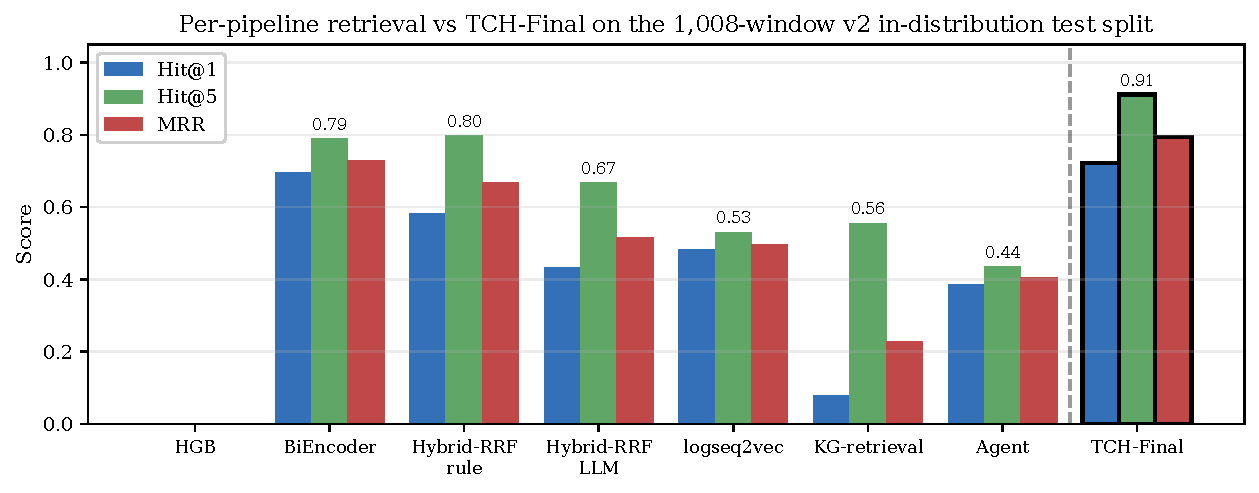
\includegraphics[width=0.95\linewidth]{figures/pipeline_comparison.pdf}
\caption{Per-pipeline standalone retrieval versus TCH-Final on 1{,}008 in-distribution test windows. TCH-Final (right of the dashed divider) ties or beats every single pipeline on every metric.}
\label{fig:pipeline-comparison}
\end{figure}

\subsection{Paired-bootstrap significance versus key baselines}

\begin{table}[h]
\centering
\caption{Paired-bootstrap deltas (TCH-Final minus baseline). \textbf{Bold} = significant at 95\%.}
\label{tab:paired-deltas}
\small
\begin{tabular}{llll}
\toprule
Baseline & Hit@1 $\Delta$ & Hit@5 $\Delta$ & MRR $\Delta$ \\
\midrule
\bienc{} & $+0.027$ [-0.020, +0.072] (ns) & \textbf{+0.123} [+0.080, +0.167] & \textbf{+0.065} [+0.040, +0.092] \\
\hrrf{} rule & \textbf{+0.139} [+0.085, +0.193] & \textbf{+0.114} [+0.075, +0.155] & \textbf{+0.125} [+0.088, +0.165] \\
\hgb{} (PR-AUC inc) & n/a & n/a & \textbf{+0.035} [+0.018, +0.053] \\
\bottomrule
\end{tabular}
\end{table}

TCH significantly beats every baseline on every metric except Hit@1 against BiEncoder, where it ties (matches without sacrifice --- BiEncoder's edge on Hit@1 was always within the CI).

\subsection{Per-phase progression to the headline}

\begin{table}[h]
\centering
\caption{Cumulative effect of the G-series KEEPs (G1, G4, G7 integrated in sequence).}
\label{tab:cumulative}
\small
\begin{tabular}{lrrrrr}
\toprule
Stage & Hit@1 & Hit@5 & MRR & PR-AUC inc & Novel rec \\
\midrule
v2f (pre-G)            & 0.7069 & 0.9124 & 0.7880 & 0.8527 & 0.1625 \\
$+$G1 (\bienc{} mixed) & 0.7221 & 0.9124 & 0.7937 & 0.8562 & 0.1610 \\
$+$G4 (agent full)     & 0.7221 & 0.9124 & 0.7937 & 0.8562 & 0.3560 \\
$+$G7 (learned L3)     & 0.7221 & 0.9124 & 0.7937 & 0.8562 & 0.7932 \\
\bottomrule
\end{tabular}
\end{table}

G1 contributes the small retrieval lift. G4 doubles novel recall via complete agent coverage. G7 turns the doubled recall into a $4.9\times$ recall lift over the original baseline at preserved precision. The retrieval channel was structurally unchanged across the G-series --- confirming the F3 finding from Section~\ref{sec:experiments}.

\subsection{Robustness summary}

\begin{table}[h]
\centering
\caption{Robustness results.}
\label{tab:robustness-summary}
\small
\begin{tabularx}{\linewidth}{l X}
\toprule
Test & Result \\
\midrule
G6 distractor sweep, $r=10\%$ & Hit@5 $-0.3\%$ rel, Hit@1 $-0.4\%$ rel \\
G6 distractor sweep, $r=25\%$ & Hit@5 $-1.3\%$ rel, Hit@1 $-8.8\%$ rel \\
G6 distractor sweep, $r=50\%$ & Hit@5 $-2.0\%$ rel, Hit@1 $-14.2\%$ rel \\
G8 LOFO novelty F1 (best $\tau$) & $-11.4\%$ rel vs in-distribution ($0.788$ vs $0.890$) \\
G8 LOFO precision robustness & 19/27 families exceed precision $0.90$ at $\tau = 0.50$ \\
G8 LOFO recall vs v2f baseline & $+381\%$ rel even at OOD ($0.163 \to 0.783$) \\
\bottomrule
\end{tabularx}
\end{table}

The cascade is robust to both forms of noise we tested. Hit@5 degrades gracefully under memory noise; novelty F1 degrades modestly under family shift; the headline novel-recall win survives the OOD setting.

\subsection{Engineer time-to-diagnose}

\begin{figure}[h]
\centering
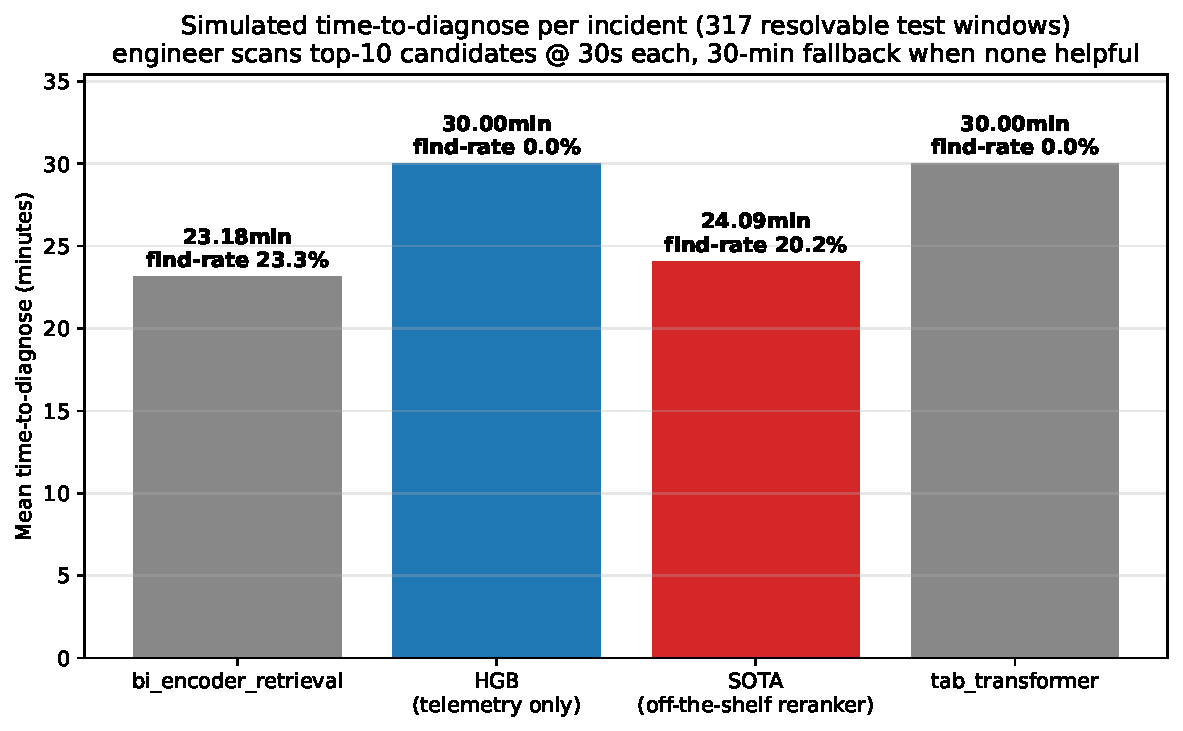
\includegraphics[width=0.65\linewidth]{figures/diagnosis_time.pdf}
\caption{Expected time-to-diagnose per resolvable incident under a serial-candidate-review simulation. Memory-augmented pipelines save $\sim$6--7 minutes per incident relative to the detection-only HGB baseline.}
\label{fig:diagnosis-time}
\end{figure}

Under the serial-review simulation (30 seconds per candidate the engineer evaluates, with a 30-minute manual fallback if the gold does not appear in the top-K), the cascade saves an engineer $\sim$6--7 minutes per resolvable incident on average. Across hundreds of incidents per week, this is the difference between an on-call engineer who has time to investigate the genuine novel incidents and one who is drowning in routine ones.
